Since finding the contact map overlap between two self-avoiding walks is NP-hard, \citet{goip99} propose ways to decompose these graphs into simpler special cases and derived polynomial time algorithms for these special cases. Before understanding these special cases, it is necessary to understand three different types of relations between pairs of edges in a contact map.
\begin{noindlist}
\item {\it Disjoint Edges:}  Let $e_1 = (v_i, v_j)$ and $e_2 = (v_{i^{\prime}}, v_{j^{\prime}})$ be two
edges in $G$. Then $e_1$ and $e_2$ are \emph{disjoint} if $(i,j) \cap (i^{\prime},j^{\prime}) = \emptyset$.
\item {\it Containing Edges:} $e_1$ \emph{contains} $e_2$ if  $(i,j) \supset (i^{\prime},j^{\prime})$.
\item {\it Overlapping Edges:} Two edges $e_1$ and $e_2$ \emph{overlap} each other if $(i,j) \cap (i^{\prime},j^{\prime}) \neq \emptyset$ and one edge does not contain the other (unless an end point is shared).
\end{noindlist}

\begin{figure}[htbp]
\begin{minipage}[b]{0.33\linewidth}
\centering
 
\centering
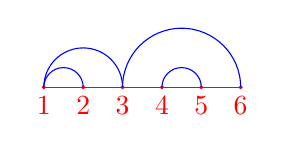
\begin{tikzpicture}[scale=0.5]


\foreach \i in {1,...,5} {
        \draw[red] (\i,1) -- (\i + 1,1)node[pos=0.0,below] {\i};
        \filldraw[red] (\i,1) circle (1pt);


 }

\draw[red] (6,1) -- (5,1)node[pos=0.0,below] {6};
\filldraw[red] (6,1) circle (1pt); 



\draw[blue, thin] (1,1) arc(180:0:0.5); 
\draw[blue, thin] (1,1) arc(180:0:1); 
\draw[blue, thin] (3,1) arc(180:0:1.5);
\draw[blue, thin] (4,1) arc(180:0:0.5);
\end{tikzpicture} 
 \vspace{0.65cm}
 \caption{Stack}
 \label{fig:Stack1}
\end{minipage}
\begin{minipage}[b]{0.33\linewidth}
\centering
 
\centering
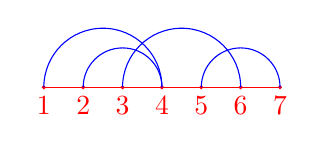
\begin{tikzpicture}[scale=0.5]


\foreach \i in {1,...,6} {
        \draw[red] (\i,1) -- (\i + 1,1)node[pos=0.0,below] {\i};
        \filldraw[red] (\i,1) circle (1pt);


 }

\draw[red] (7,1) -- (6,1)node[pos=0.0,below] {7};
\filldraw[red] (7,1) circle (1pt); 



\draw[blue, thin] (1,1) arc(180:0:1.5); 
\draw[blue, thin] (2,1) arc(180:0:1);
\draw[blue, thin] (3,1) arc(180:0:1.5);
\draw[blue, thin] (5,1) arc(180:0:1);
\end{tikzpicture} 
 \vspace{0.65cm}
 \caption{Queue}
 \label{fig:Queue}
\end{minipage}
\begin{minipage}[b]{0.33\linewidth}
\centering
 
\centering
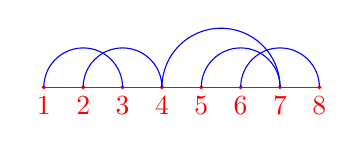
\begin{tikzpicture}[scale=0.5]


\foreach \i in {1,...,7} {
        \draw[red] (\i,1) -- (\i + 1,1)node[pos=0.0,below] {\i};
        \filldraw[red] (\i,1) circle (1pt);


 }

\draw[red] (8,1) -- (7,1)node[pos=0.0,below] {8};
\filldraw[red] (8,1) circle (1pt); 



\draw[blue, thin] (1,1) arc(180:0:1); 
\draw[blue, thin] (2,1) arc(180:0:1);
\draw[blue, thin] (4,1) arc(180:0:1.5);
\draw[blue, thin] (5,1) arc(180:0:1);
\draw[blue, thin] (6,1) arc(180:0:1);
\end{tikzpicture} 
 \vspace{0.65cm}
 \caption{Staircase}
 \label{fig:Staircase}
\end{minipage}
\end{figure}

Based on the above relations, \citet{goip99} propose three simpler graphs as follows:
\begin{noindlist}
\item {\it Stack:} A stack is defined as the contact map $(V,E)$ where if $e_1$ and $e_2$ are two edges in the contact map then either they contain one another, are disjoint or overlap at one end point.
\item {\it Queue:} A queue is defined as the contact map $(V,E)$ where if $e_1$ and $e_2$ are two edges in the contact map then they do not contain one another unless they share one end-point.
\item {\it Staircase:} A staircase is a special case of queue in which there are sets of mutually overlapping intervals such that either no two intervals in the different sets meet, or at most two of them overlap at an end-point.
\end{noindlist}
These graphs are illustrated in Figs. \ref{fig:Stack1}, \ref{fig:Queue} and \ref{fig:Staircase}. The proofs corresponding to the computation of contact map overlap for all of these special cases have similar structure and use dynamic programming. Some noteworthy results are presented in the following sections.

\subsection{$O(n^4)$ algorithm for maximum CMO of $2$-stack and degree-$2$ contact map}

Let $\text{co}(G_1,G_2)$ denote the overlap between $G_1$, a degree-2 stack of $n_1$ vertices and $G_2$, a degree-2 contact map of $n_2$ vertices. Now, since it is tabulated using dynamic programming, the subproblems are formed by computing the contact overlap of subgraphs like ${G_1}_{(v_a,v_b)}$ and ${G_2}_{(u_c,u_d)}$ where $v_1 \leq v_a < v_b \leq v_{n_1}$ and $1 \leq u_c < u_d \leq u_{n_2}$. There are few rules that are followed for computing the contact overlap of these two subgraphs recursively. The first one is that if two edges meet $v_b$(or $u_d$) then one must omit the lower first coordinate in each case. These are denoted by ${G_1}_{\hat{(v_a,v_b)}}$ or ${G_2}_{\hat{(u_c,u_d)}}$. Another rule is that an edge with the lowest end-point in one graph is mapped to the edge with the lowest endpoint in the other. These graphs can be denoted as $\text{co}({G_1}_{(v_a,v_b)}, {G_2}_{(u_c,u_d)})^l$. Similarly, edges with the highest end point will be mapped to one another. These graphs are denoted as $\text{co}({G_1}_{(v_a,v_b)}, {G_2}_{(u_c,u_d)})^h$. If both the edges are mapped, then the graph is denoted by $\text{co}({G_1}_{(v_a,v_b)}, {G_2}_{(u_c,u_d)})^{lh}$. The optimum contact map can be computed as follows:
\begin{eqnarray}
\label{sqs1}
\text{co}(G_1,G_2) = \max\{\text{co}({G_1}_{(v_1,v_{n_1})}, {G_2}_{(u_1,u_{n_2})})^h,\text{co}({G_1}_{\hat{(v_1,v_{n_1})}}, {G_2}_{(u_1,u_{n_2})})^h,\text{co}({G_1}_{(v_1,v_{n_1})}, \cap \nonumber \\ {G_2}_{\hat{(u_1,u_{n_2})}})^h,\text{co}({G_1}_{\hat{(v_1,v_{n_1})}}, {G_2}_{\hat{(u_1,u_{n_2})}})^h,\text{co}({G_1}_{(v_1,v_{(n_1-1)})}, {G_2}_{(u_1,u_{n_2})}),\text{co}({G_1}_{(v_1,v_{n_1})}, {G_2}_{(u_1,u_{(n_2-1)})}\}
\end{eqnarray}

\begin{figure}[htbp]
\begin{minipage}[b]{0.50\linewidth}
\centering
 
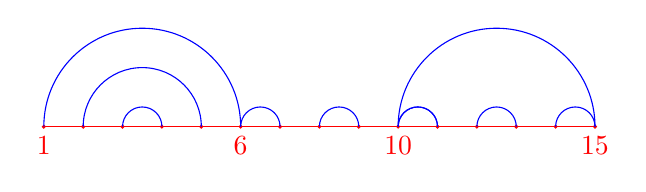
\begin{tikzpicture}[scale=0.5]
\centering
\label{staircasedecompisition}

\foreach \i in {1,...,14} {
        \draw[red] (\i,1) -- (\i + 1,1);
        \filldraw[red] (\i,1) circle (1pt);
 }
\draw[red] (15,1) -- (14,1)node[pos=0.0,below] {15};
\draw[red] (10,1) -- (9,1)node[pos=0.0,below] {10};
\draw[red] (6,1) -- (5,1)node[pos=0.0,below] {6};
\draw[red] (1,1) -- (2,1)node[pos=0.0,below] {1};
\filldraw[red] (15,1) circle (1pt);

\draw[blue, thin] (1,1) arc(180:0:2.5);
\draw[blue, thin] (2,1) arc(180:0:1.5);
\draw[blue, thin] (3,1) arc(180:0:0.5);
\draw[blue, thin] (6,1) arc(180:0:0.5);
\draw[blue, thin] (8,1) arc(180:0:0.5);
\draw[blue, thin] (10,1) arc(180:0:2.5);
\draw[blue, thin] (10,1) arc(180:0:0.5);
\draw[blue, thin] (10,1) arc(180:0:0.5);
\draw[blue, thin] (12,1) arc(180:0:0.5);
\draw[blue, thin] (14,1) arc(180:0:0.5);

\end{tikzpicture}
 \vspace{0.65cm}
 \caption{${G_1}_{(1,15)}$}
 \label{fig:$S_{(1,15)}$}
\end{minipage}
\begin{minipage}[b]{0.50\linewidth}
\centering
 
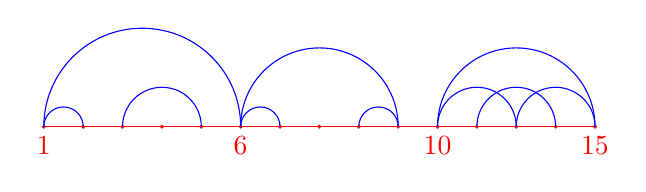
\begin{tikzpicture}[scale=0.5]
\centering
\label{staircasedecompisition}

\foreach \i in {1,...,14} {
        \draw[red] (\i,1) -- (\i + 1,1);
        \filldraw[red] (\i,1) circle (1pt);
 }
\draw[red] (15,1) -- (14,1)node[pos=0.0,below] {15};
\draw[red] (11,1) -- (10,1)node[pos=0.0,below] {10};
\draw[red] (6,1) -- (5,1)node[pos=0.0,below] {6};
\draw[red] (1,1) -- (2,1)node[pos=0.0,below] {1};
\filldraw[red] (15,1) circle (1pt);

\draw[blue, thin] (1,1) arc(180:0:2.5);
\draw[blue, thin] (1,1) arc(180:0:0.5);
\draw[blue, thin] (3,1) arc(180:0:1);
\draw[blue, thin] (6,1) arc(180:0:2);
\draw[blue, thin] (6,1) arc(180:0:0.5);
\draw[blue, thin] (9,1) arc(180:0:0.5);
\draw[blue, thin] (11,1) arc(180:0:2);
\draw[blue, thin] (11,1) arc(180:0:1);
\draw[blue, thin] (13,1) arc(180:0:1);
\draw[blue, thin] (12,1) arc(180:0:1);


\end{tikzpicture}
 \vspace{0.65cm}
 \caption{${G_2}_{(1,15)}$}
 \label{fig:$G_{(1,15)}$}
\end{minipage}
\end{figure}

Let us consider two subgraphs in Figs. \ref{fig:$S_{(1,15)}$} and \ref{fig:$G_{(1,15)}$}. Recursively,
the contact map of the two are given as:
\begin{eqnarray}
\label{sqs2}
\text{co}({G_1}_{(1,15)}, {G_2}_{(1,15)})^{lh} = 2+ \text{co}({G_1}_{(2,5)}, {G_2}_{(2,5)}) + \max\{\text{co}({G_1}_{(6,10)}, {G_2}_{(6,11)})^l,\text{co}({G_1}_{(7,10)}, {G_2}_{(7,11)})\} \cap \nonumber \\
+ \max \{\text{co}({G_1}_{(10,14)}, {G_2}_{(11,14)})^l,\text{co}({G_1}_{(11,15)}, {G_2}_{(12,15)})^h,\text{co}({G_1}_{(11,14)}, {G_2}_{(12,14)})\}
\end{eqnarray}
Here, one can see that node $1$ and node $15$ of each graph are matched for which $2$ is already counted in the calculation. The remaining calculation is for the intermediate edges. One subproblem in such setting is calculation of the number of matchings between nodes $2$ and $5$ of each graph. The next part of the equation computes the number of edges matching between node $6$ and $10$ in graph ${G_1}_{(1,15)}$ and $6$ and $11$ in graph ${G_2}_{(1,15)}$. It would take the maximum number of edges matched in two scenarios - one would be if the edge with lowest end-point at node $6$ matches with the lowest end point at node $6$ and the other would be to calculate the total number of edges matched from node $7$ to node $10$ in one and from node $7$ to node $11$ in the other. Matching at node $10$ and $11$ is excluded because there are no incoming edges at them. The third part of the calculation also follows the same order.

If $G_1$ is of size n, then from Eq. \ref{sqs1}, it can be seen that the total number of entries in the table is $O(n^4)$ and each table entry takes $O(1)$ time to compute. So the total time taken to compute all the entries is $O(n^4)$.

\subsection{$O(n^3)$ algorithm for maximum CMO of $2$-staircase and degree-$2$ contact map}

Considering $G_1$ to be a degree-2 staircase containing $n_1$ vertices and $G_2$ to be any degree-2 graph containing $n_2$ vertices, the computation of $\text{co}(G_1,G_2)$ is done again using a dynamic programming method. Firstly, the edges in $G_1$ and $G_2$ are numbered according to the ascending order of their right end points. If there are two edges which share the same right end point, the edge with the higher lowest end point is given higher number. A table is constructed with these two graphs having these $3$ indices - an edge $e_i$ from $G_1$, an edge $f_j$ from $G_2$ and the next entry is either a blank denoted by ``-" or contains a higher edge $f_{j^\prime}$ of $G_2$ whose interval overlaps edge $f_j$ at more than one points. Thus the table entries contain a contact overlap between a subgraph of $G_1$ denoted by ${G_1}_{e_i}$ which consists of all edges smaller than or equal to $e_i$ and a subgraph of $G_2$ denoted by ${G_2}_{(f_j,{f_{j^\prime}})}$ which consists of all edges smaller than or equal to $f_j$. There is a constraint of the above contact map which states that all edges of ${G_2}_{(f_j,{f_{j^\prime}})}$ that overlap $f_j$ also overlaps $f_{j^\prime}$ at more than one point. It is reasonable to say now that $f_{j^\prime}$ being the edge which overlaps $f_j$ at more than one point also matches an edge overlapping $e_i$. Also like the proof in the earlier case, if the highest endpoints of $e_i$ and $f_j$ map to each other, the corresponding contact map overlap is denoted by $\text{co}({G_1}_{e_i}, {G_2}_{(f_j,{f_{j^\prime}})})^h$.

Assuming that $G_1$ and $G_2$ contain $n_1$ and $n_2$ number of edges, the contact overlap between the two graphs is given by:
\begin{eqnarray}
\label{sqs3}
\text{co}(G_1,G_2) = \max\{\text{co}({G_1}_{n_1}, {G_2}_{({n_2},-)})^h, \text{co}({G_1}_{({n_1}-1)}, {G_2}_{({n_2},-)}),\text{co}({G_1}_{n_1}, {G_2}_{({n_2}-1,-)})\}
\end{eqnarray}
The subproblem $\text{co}({G_1}_{n_{e_1}}, {G_2}_{({n_{e_2}},-)})^h$ here which would recursively operate is also calculated similarly to the ones in the previous algorithm. The edges would be selected as those edges which overlap $e_i$ or $f_j$(in the staircase it would always be $e_({i-1})$) and the third entry would either be absent or would be the edge that overlaps $e_i$ or $f_j^\prime$ at more than one point. Now, considering all the columns in the table entries, the total number of entries are $O(n^3)$(if n is the number of vertices in $G_1$) and each table entry takes $O(1)$ time to compute. So the total time taken to compute all the entries is $O(n^3)$.

Now, any RNA structure (except one) is known to be decomposable into two degree-1 stacks \citep{goip99}. Any of these degree-1 stacks will have half of the edges that must be in the optimal alignment. So when this contact map of the RNA structure is optimized with any other contact map using the algorithm used for stack it can be guaranteed that the output will have at least half of edges mapped in the optimal solution. Thus one obtains a 2-approximation algorithm for constructing a contact map between two RNA structures. In the case of a queue, finding the contact map overlap between a queue and another contact map is NP-complete.  The approximation algorithm for queues are not shown separately because each queue can be decomposed into two staircases and following the same logic described above, there is a 2-approximation algorithm for computing the contact map overlap of a queue and another contact map.

The best results for approximation algorithm are obtained for a special case of contact map called augmented staircase. An \emph{augmented staircase} is a contact map which can be decomposed into a staircase and a stack with the constraint that for every stack edge and for every staircase edge, the interval formed by the edges are disjoint, overlap at an end point or the interval formed by the staircase edge contains the interval formed by the stack edge. The best polynomial results were obtained by computing the contact overlap between an augmented staircase and any degree-2 contact map.

\subsection{$O(n^6)$ algorithm for maximum CMO of augmented $2$-staircase and degree-$2$ contact map}

This algorithm builds the same way as the staircase algorithm and uses the stack algorithm as a subroutine. Let $G_1$ be a degree-2 augmented staircase of $n_1$ vertices and $G_2$ any degree-2 graph of $n_2$ vertices. Here edges in $G_1$ and $G_2$ are numbered according to ascending order of their right end points. $G_1$ can be decomposed into a staircase $T$ and a stack $S$. The stack algorithm is used to compute the table entries for the comparison between subgraphs of $S$ and subgraphs of $G_2$. In $T$, if two edges share the same right end-point, the edge with the higher left end point is numbered higher. The table here has four entries: $e=(v_i,v_j)$ from $T$, $f=(u_k,u_l)$ from $G_2$. The other two table entries are either empty or a higher edge $e^\prime$ of $T$ which overlaps with $e$ at more than one point and an edge $f^\prime$ of $G_2$ whose interval overlaps with $f$ at more than one point. The above table entry contains the constrained contact overlap between the subgraph $G_1$ denoted ${G_1}_{(e,{e^\prime})}$, consisting of all the edges less than or equal to $e$ and excluding the edges in $S$ which are in the interval formed by $e$ and $e^\prime$, and subgraph of $G_2$ denoted by ${G_2}_{(f,{f^\prime})}$, consisting of all edges less than or equal to $f$. Here  the constraint is that $e$ must map to $f$ and the mapped edges of ${G_2}_{(f,{f^\prime})}$ which overlap $f$ overlaps $f^\prime$ at more than a point. The contact overlap of $G_1$ and $G_2$ is thus given by:
\begin{eqnarray}
\label{sqs4}
\text{co}(G_1,G_2) = \max\{\text{co}(S,G),\max_{e \in T, f \in G_2}\{\text{co}({G_1}_{(e,-)} {G_2}_{(f,-)}) + s(j,l)\}.
\end{eqnarray}
\begin{eqnarray}
where, s(j,l) = \begin{cases}
    \max\{co(S_{(j,n_1)},{G_2}_{(l,{n_2})})^l,co(S_{(j+1,n_1)},{G_2}_{(l+1,n_2)})\}, & \\ \text{edges of $S$ and $G_2$ meet $j$, $l$ as left end points}.\\
    co(S_{(j+1,n_1),{G_2}_{(l+1,n_2)}}), \text{otherwise}.
  \end{cases}
\end{eqnarray}
The optimal bijection maps the highest edges of $T$ to an edge of $G_2$ or there is no such edge. The recursion maps the next highest edge in the subgraph of $T$ to $G_2$. So, if $G_1$is of size n, the total number of table entries is $O(n^4)$ and each entry takes $O(n^2)$ time to compute. Hence, the total time to compute the contact overlap between an augmented staircase and any degree-2 graph is $O(n^6)$. 